\documentclass[11pt]{article}
\usepackage[margin=.82in]{geometry}
\usepackage{amsmath,amssymb,booktabs,array,tabularx,graphicx,enumitem,hyperref,microtype,xcolor,xspace,float}
\hypersetup{colorlinks=true,linkcolor=blue!45!black,urlcolor=blue!45!black,hypertexnames=false}
\newcommand{\pra}{\textsc{PRA}\xspace}
\newcommand{\kv}{K/V\xspace}
\newcommand{\code}[1]{\texttt{#1}}
\title{Generated Summaries as Retrieval Indices for Progressive Retrieval Attention\\
\large Compact Addresses and Fixed-Budget Competition}
\author{Jorge Sim\~ao}
\date{August 2026}
\newcommand{\PaperThreeOneMultiValidationN}{8}
\newcommand{\PaperThreeOneMultiTestN}{24}
\newcommand{\PaperThreeOneMultiK}{4}
\newcommand{\PaperThreeOneSummaryUniqueQasper}{2}
\newcommand{\PaperThreeOneSummaryUniqueMusique}{3}
\newcommand{\PaperThreeOneEvidenceKeyRetention}{0.276}
\newcommand{\PaperThreeOneEvidenceKeyCorrelation}{0.442}
\newcommand{\PaperThreeOneMusiqueReservedRecall}{0.719}
\newcommand{\PaperThreeOneMusiqueReservedDelta}{+0.073}
\newcommand{\PaperThreeOneMusiqueReservedLow}{-0.115}
\newcommand{\PaperThreeOneMusiqueReservedHigh}{+0.260}
\newcommand{\PaperThreeOneHotpotRrfBase}{1.000}
\newcommand{\PaperThreeOneHotpotRrfFull}{1.000}
\newcommand{\PaperThreeOneHotpotRrfSummaryDelta}{+0.000}
\newcommand{\PaperThreeOneHotpotRrfLow}{+0.000}
\newcommand{\PaperThreeOneHotpotRrfHigh}{+0.000}
\newcommand{\PaperThreeOneHotpotRrfWins}{0}
\newcommand{\PaperThreeOneHotpotRrfTies}{4}
\newcommand{\PaperThreeOneHotpotRrfLosses}{0}
\newcommand{\PaperThreeOneHotpotRoundRobinBase}{1.000}
\newcommand{\PaperThreeOneHotpotRoundRobinFull}{1.000}
\newcommand{\PaperThreeOneHotpotRoundRobinSummaryDelta}{+0.000}
\newcommand{\PaperThreeOneHotpotRoundRobinLow}{+0.000}
\newcommand{\PaperThreeOneHotpotRoundRobinHigh}{+0.000}
\newcommand{\PaperThreeOneHotpotRoundRobinWins}{0}
\newcommand{\PaperThreeOneHotpotRoundRobinTies}{4}
\newcommand{\PaperThreeOneHotpotRoundRobinLosses}{0}
\newcommand{\PaperThreeOneHotpotAgreementBase}{1.000}
\newcommand{\PaperThreeOneHotpotAgreementFull}{1.000}
\newcommand{\PaperThreeOneHotpotAgreementSummaryDelta}{+0.000}
\newcommand{\PaperThreeOneHotpotAgreementLow}{+0.000}
\newcommand{\PaperThreeOneHotpotAgreementHigh}{+0.000}
\newcommand{\PaperThreeOneHotpotAgreementWins}{0}
\newcommand{\PaperThreeOneHotpotAgreementTies}{4}
\newcommand{\PaperThreeOneHotpotAgreementLosses}{0}
\newcommand{\PaperThreeOneHotpotFusionBase}{1.000}
\newcommand{\PaperThreeOneHotpotFusionFull}{1.000}
\newcommand{\PaperThreeOneHotpotFusionSummaryDelta}{+0.000}
\newcommand{\PaperThreeOneHotpotFusionLow}{+0.000}
\newcommand{\PaperThreeOneHotpotFusionHigh}{+0.000}
\newcommand{\PaperThreeOneHotpotFusionWins}{0}
\newcommand{\PaperThreeOneHotpotFusionTies}{4}
\newcommand{\PaperThreeOneHotpotFusionLosses}{0}
\newcommand{\PaperThreeOneQasperRrfBase}{0.588}
\newcommand{\PaperThreeOneQasperRrfFull}{0.475}
\newcommand{\PaperThreeOneQasperRrfSummaryDelta}{-0.113}
\newcommand{\PaperThreeOneQasperRrfLow}{-0.375}
\newcommand{\PaperThreeOneQasperRrfHigh}{+0.037}
\newcommand{\PaperThreeOneQasperRrfWins}{1}
\newcommand{\PaperThreeOneQasperRrfTies}{6}
\newcommand{\PaperThreeOneQasperRrfLosses}{1}
\newcommand{\PaperThreeOneQasperRoundRobinBase}{0.575}
\newcommand{\PaperThreeOneQasperRoundRobinFull}{0.588}
\newcommand{\PaperThreeOneQasperRoundRobinSummaryDelta}{+0.013}
\newcommand{\PaperThreeOneQasperRoundRobinLow}{+0.000}
\newcommand{\PaperThreeOneQasperRoundRobinHigh}{+0.038}
\newcommand{\PaperThreeOneQasperRoundRobinWins}{1}
\newcommand{\PaperThreeOneQasperRoundRobinTies}{7}
\newcommand{\PaperThreeOneQasperRoundRobinLosses}{0}
\newcommand{\PaperThreeOneQasperAgreementBase}{0.575}
\newcommand{\PaperThreeOneQasperAgreementFull}{0.475}
\newcommand{\PaperThreeOneQasperAgreementSummaryDelta}{-0.100}
\newcommand{\PaperThreeOneQasperAgreementLow}{-0.375}
\newcommand{\PaperThreeOneQasperAgreementHigh}{+0.075}
\newcommand{\PaperThreeOneQasperAgreementWins}{1}
\newcommand{\PaperThreeOneQasperAgreementTies}{6}
\newcommand{\PaperThreeOneQasperAgreementLosses}{1}
\newcommand{\PaperThreeOneQasperFusionBase}{0.588}
\newcommand{\PaperThreeOneQasperFusionFull}{0.537}
\newcommand{\PaperThreeOneQasperFusionSummaryDelta}{-0.050}
\newcommand{\PaperThreeOneQasperFusionLow}{-0.188}
\newcommand{\PaperThreeOneQasperFusionHigh}{+0.037}
\newcommand{\PaperThreeOneQasperFusionWins}{1}
\newcommand{\PaperThreeOneQasperFusionTies}{6}
\newcommand{\PaperThreeOneQasperFusionLosses}{1}
\newcommand{\PaperThreeOneTwoWikiRrfBase}{1.000}
\newcommand{\PaperThreeOneTwoWikiRrfFull}{0.917}
\newcommand{\PaperThreeOneTwoWikiRrfSummaryDelta}{-0.083}
\newcommand{\PaperThreeOneTwoWikiRrfLow}{-0.250}
\newcommand{\PaperThreeOneTwoWikiRrfHigh}{+0.000}
\newcommand{\PaperThreeOneTwoWikiRrfWins}{0}
\newcommand{\PaperThreeOneTwoWikiRrfTies}{3}
\newcommand{\PaperThreeOneTwoWikiRrfLosses}{1}
\newcommand{\PaperThreeOneTwoWikiRoundRobinBase}{1.000}
\newcommand{\PaperThreeOneTwoWikiRoundRobinFull}{0.917}
\newcommand{\PaperThreeOneTwoWikiRoundRobinSummaryDelta}{-0.083}
\newcommand{\PaperThreeOneTwoWikiRoundRobinLow}{-0.250}
\newcommand{\PaperThreeOneTwoWikiRoundRobinHigh}{+0.000}
\newcommand{\PaperThreeOneTwoWikiRoundRobinWins}{0}
\newcommand{\PaperThreeOneTwoWikiRoundRobinTies}{3}
\newcommand{\PaperThreeOneTwoWikiRoundRobinLosses}{1}
\newcommand{\PaperThreeOneTwoWikiAgreementBase}{0.917}
\newcommand{\PaperThreeOneTwoWikiAgreementFull}{0.917}
\newcommand{\PaperThreeOneTwoWikiAgreementSummaryDelta}{+0.000}
\newcommand{\PaperThreeOneTwoWikiAgreementLow}{+0.000}
\newcommand{\PaperThreeOneTwoWikiAgreementHigh}{+0.000}
\newcommand{\PaperThreeOneTwoWikiAgreementWins}{0}
\newcommand{\PaperThreeOneTwoWikiAgreementTies}{4}
\newcommand{\PaperThreeOneTwoWikiAgreementLosses}{0}
\newcommand{\PaperThreeOneTwoWikiFusionBase}{1.000}
\newcommand{\PaperThreeOneTwoWikiFusionFull}{1.000}
\newcommand{\PaperThreeOneTwoWikiFusionSummaryDelta}{+0.000}
\newcommand{\PaperThreeOneTwoWikiFusionLow}{+0.000}
\newcommand{\PaperThreeOneTwoWikiFusionHigh}{+0.000}
\newcommand{\PaperThreeOneTwoWikiFusionWins}{0}
\newcommand{\PaperThreeOneTwoWikiFusionTies}{4}
\newcommand{\PaperThreeOneTwoWikiFusionLosses}{0}
\newcommand{\PaperThreeOneMusiqueRrfBase}{0.573}
\newcommand{\PaperThreeOneMusiqueRrfFull}{0.573}
\newcommand{\PaperThreeOneMusiqueRrfSummaryDelta}{+0.000}
\newcommand{\PaperThreeOneMusiqueRrfLow}{+0.000}
\newcommand{\PaperThreeOneMusiqueRrfHigh}{+0.000}
\newcommand{\PaperThreeOneMusiqueRrfWins}{0}
\newcommand{\PaperThreeOneMusiqueRrfTies}{8}
\newcommand{\PaperThreeOneMusiqueRrfLosses}{0}
\newcommand{\PaperThreeOneMusiqueRoundRobinBase}{0.542}
\newcommand{\PaperThreeOneMusiqueRoundRobinFull}{0.615}
\newcommand{\PaperThreeOneMusiqueRoundRobinSummaryDelta}{+0.073}
\newcommand{\PaperThreeOneMusiqueRoundRobinLow}{+0.000}
\newcommand{\PaperThreeOneMusiqueRoundRobinHigh}{+0.167}
\newcommand{\PaperThreeOneMusiqueRoundRobinWins}{2}
\newcommand{\PaperThreeOneMusiqueRoundRobinTies}{6}
\newcommand{\PaperThreeOneMusiqueRoundRobinLosses}{0}
\newcommand{\PaperThreeOneMusiqueAgreementBase}{0.604}
\newcommand{\PaperThreeOneMusiqueAgreementFull}{0.573}
\newcommand{\PaperThreeOneMusiqueAgreementSummaryDelta}{-0.031}
\newcommand{\PaperThreeOneMusiqueAgreementLow}{-0.094}
\newcommand{\PaperThreeOneMusiqueAgreementHigh}{+0.000}
\newcommand{\PaperThreeOneMusiqueAgreementWins}{0}
\newcommand{\PaperThreeOneMusiqueAgreementTies}{7}
\newcommand{\PaperThreeOneMusiqueAgreementLosses}{1}
\newcommand{\PaperThreeOneMusiqueFusionBase}{0.542}
\newcommand{\PaperThreeOneMusiqueFusionFull}{0.573}
\newcommand{\PaperThreeOneMusiqueFusionSummaryDelta}{+0.031}
\newcommand{\PaperThreeOneMusiqueFusionLow}{+0.000}
\newcommand{\PaperThreeOneMusiqueFusionHigh}{+0.094}
\newcommand{\PaperThreeOneMusiqueFusionWins}{1}
\newcommand{\PaperThreeOneMusiqueFusionTies}{7}
\newcommand{\PaperThreeOneMusiqueFusionLosses}{0}


\begin{document}
\maketitle

\begin{abstract}
Long-memory systems must decide both \emph{what to retrieve} and \emph{how the
model will consume it}. Progressive Retrieval Attention (\pra) separates these
problems: compact address views discover source identities, then selected
identities resolve to unchanged source-derived keys and values. This boundary
makes generated summaries plausible retrieval indices without making summary
text the evidence. We implement an identity-preserving summary sidecar and
compare it with lexical, typed extractive, and learned native-QK addresses on
identity-disjoint HotpotQA, QASPER, 2WikiMultiHopQA, and MuSiQue cohorts.
Standalone summaries raise QASPER recall from $0.350$ to $0.513$ over a native
mean-key baseline, but tie or regress elsewhere. The stricter fixed-budget test
asks whether a summary remains useful after stronger views compete for the same
four materialization slots. Under validation-frozen reciprocal-rank fusion,
adding the summary changes held-out recall by
$\PaperThreeOneHotpotRrfSummaryDelta$, $\PaperThreeOneQasperRrfSummaryDelta$,
$\PaperThreeOneTwoWikiRrfSummaryDelta$, and
$\PaperThreeOneMusiqueRrfSummaryDelta$, respectively. No positive paired
interval excludes zero. Summaries nevertheless recover
\PaperThreeOneSummaryUniqueQasper{} QASPER and
\PaperThreeOneSummaryUniqueMusique{} MuSiQue evidence parents missed by every
other single channel, so the issue is admission under a fixed budget rather
than complete redundancy. A controlled omission benchmark further shows that
fluent summaries can lose low-salience entities and aliases needed by future
queries. The central result is therefore that standalone value is not marginal
value: the supported default is lexical, extractive, and QK addressing, while
summary addresses remain optional until a selective controller establishes a
reproducible gain.
\end{abstract}

\section{Introduction}

Long-context systems face two different problems that are often collapsed into one. The first is \emph{discovery}: deciding which old source chunks might matter to the current query. The second is \emph{consumption}: presenting the corresponding information to the language model in the representation it expects. \pra treats them as separate stages. A small resident index performs discovery; only selected source identities cause native keys and values to enter the active attention set.

This paper asks whether generated natural language can serve as that resident
index. Consider a report whose main topic is equipment maintenance but whose
appendix records the alias ``Northglass.'' A fluent summary will probably
preserve the main topic. A later query about the alias, however, needs that
seemingly minor detail. The summary can be concise, faithful, and useful to a
reader while still being a poor retrieval address. Ordinary summarization
preserves what appears salient now; routing must preserve discriminators for
queries that are not known when the index is built.

We evaluate that tension without turning the experiment into text retrieval-augmented generation. Each generated address remains bound to an exact source URI, chunk identifier, token span, and source hash. A successful match materializes the original source chunk's unchanged native \kv; summary text never becomes answer evidence. The implementation therefore tests lossy discovery while preserving native consumption.

The principal finding is mixed but useful. A frozen 0.6B retrieval summary
raises held-out QASPER recall from $0.350$ to $0.513$, but an inherited rank-16
QK selector reaches $0.775$. More importantly, the new multi-index experiment
shows that standalone value is not marginal value. A summary can recover a
candidate missed by another channel and still reduce final recall if it
displaces stronger candidates from a four-slot palette. Controlled
low-salience targets explain the pressure: generated addresses often omit the
exact entity, alias, date, or rare string that makes a chunk reachable. A cheap
extractive index preserves these addresses more reliably.

This study contributes five concrete results:
\begin{enumerate}[leftmargin=*]
\item an identity-safe summary sidecar whose output cannot leak into native-\kv materialization;
\item a matched-budget comparison across four natural datasets and inherited lexical and learned-QK baselines;
\item controlled omission and equal-token facet experiments that isolate coverage from fluency;
\item a fixed-budget multi-index comparison of round-robin, reserved-slot,
agreement, reciprocal-rank, and normalized-score admission; and
\item measured index, ingestion, routing, and amortization costs that prevent compact storage from being confused with cheap operation.
\end{enumerate}

The remainder of the paper introduces the identity-safe address boundary,
freezes the evaluation protocol, and then moves from standalone retrieval to
omission, fixed-budget competition, and cost. Related systems and limitations
place the negative marginal result in context. Detailed scorer, cache, facet,
admission, and reproducibility material appears in the appendices.

\section{Summary addresses in PRA}

Earlier work in the \pra series narrows the question. Paper 2.5 found that iterative associative closure can expose controlled bridges but does not reliably improve natural multihop retrieval. Paper 2.6 found lexical and semantic channels to be complementary. Paper 2.7 showed that query faceting is not automatically beneficial. Paper 2.8 found that learned low-rank native-QK routing can improve selected semantic cohorts while BM25 remains strong for lexical evidence. Paper 2.9 found no reliable held-out gain from short temporal query pooling. Paper 3 then separated conceptual selection from physical native-\kv materialization.

Paper 3.1 changes only the representation used for discovery. It does not
compress active \kv, rewrite source state, or answer from summaries. This
distinction also separates the method from conventional text RAG
\cite{lewis2020rag}: retrieved language is an address that resolves to
model-native evidence, not the evidence placed in the prompt.

The result is best understood as a typed-index question. Source BM25 preserves explicit strings. A generated summary can normalize paraphrases and relations. Learned QK features preserve host-model geometry. These representations fail differently, so the scientific question is not whether one replaces all others, but whether generated language adds enough complementary discovery to justify its ingestion cost.

\subsection{An address backed by native evidence}

Let source chunk $C_i$ occupy token span $[a_i,b_i)$ within source URI $u_i$. Ingestion generates a bounded address
\[
S_i=f_\theta(C_i),
\]
where $f_\theta$ is frozen in the main study. The persistent record is
\[
R_i=(u_i, i, a_i,b_i,h(C_i),S_i),
\]
where $h(C_i)$ is a SHA-256 digest of the exact source text. The first five fields form the native-memory identity. The final field is replaceable routing metadata.

For query $Q$, a scorer $g$ assigns one score per record,
\[
r_i=g(Q,S_i).
\]
The router chooses the top $k$ identities $\mathcal I_k$. Materialization then discards $S_i$ and requests
\[
\mathcal M(Q)=\{(u_i,i,a_i,b_i,h(C_i)):i\in\mathcal I_k\}.
\]
The unchanged materializer resolves those identities to source-derived native \kv. This projection is intentionally one-way: the native-\kv request type has no summary field.

\begin{figure}[t]
\centering
\fbox{\begin{minipage}{0.91\linewidth}
\centering
source chunk $C_i$ $\rightarrow$ frozen generator $f_\theta$ $\rightarrow$ summary address $S_i$\\[3pt]
$\downarrow$ stable URI, chunk, span, and source hash $\hspace{25mm}\downarrow$ persistent routing sidecar\\[3pt]
query $Q$ $\rightarrow$ lexical / extractive / summary / native-QK views $\rightarrow$ selected identities $\mathcal I_k$\\[3pt]
$\downarrow$ summary text is dropped\\[3pt]
unchanged native-\kv materializer $\rightarrow$ selected source-derived $K_i,V_i$ $\rightarrow$ direct + memory attention
\end{minipage}}
\caption{The summary is a lossy address. Selection resolves back to an immutable source identity before native keys and values are materialized.}
\label{fig:architecture}
\end{figure}

\subsection{Persistent sidecar and cache safety}

The implementation lives in \code{src/pra\_hf/summary\_index.py}. \code{SummaryIndexRecord} stores the immutable identity beside generated summary text or independently scored facets. \code{native\_kv\_request()} removes all lossy text. \code{assert\_source\_alignment()} compares the full URI, span, and hash set with the inherited native-memory registry before evaluation.

Generation is deterministic and resumable. Cache reuse is content-based, but
every hit is rebound to the requesting immutable identity before it can reach
the materializer. Appendix~\ref{app:cache} gives the cache key and provenance
checks.

\subsection{Scorers are separate from summaries}

Summary quality and query matching are independent variables. We therefore
score the same generated address with exact overlap, BM25, frozen MiniLM, and a
validation-frozen lexical--embedding fusion. This separation prevents a good
generator from being credited for a better scorer, or vice versa. The complete
scorer frontier and fusion equation appear in Appendix~\ref{app:frontier}.

\subsection{One backing memory, multiple address views}

The next iteration gives every parent identity four aligned address views:
source BM25 ($L$), a deterministic entity/rare-term sidecar ($E$), the frozen
generated summary policy ($S$), and the five-seed rank-16 native-QK selector
($QK$). The typed extractive record retains separately detected entities,
optional aliases, numbers and dates, corpus-rare terms, high-IDF bigrams, and
relation terms. Its extraction is deterministic but not claimed to be
semantically lossless.

Each channel produces a score and rank for the same parent $i$. The router may
combine these addresses, but the final set remains bounded:
\[
\mathcal I_K=\operatorname{Admit}_K
  (r^L,r^E,r^S,r^{QK}),\qquad |\mathcal I_K|\le K.
\]
We test rank round-robin, fixed slot reservations, agreement priority,
reciprocal rank fusion (RRF), and min--max normalized score fusion. RRF uses
\[
r_i^{\mathrm{RRF}}=\sum_{c\in\mathcal C}\frac{1}{d+\operatorname{rank}_c(i)}.
\]
The small choice $d\in\{10,60\}$ and five interpretable score-weight templates
are frozen separately by dataset and channel combination on validation
identities. Every test row retains each selected parent's score and rank from
every participating channel. Sidecar representations are then discarded, and
the selected integer parent identities enter the unchanged native-\kv request
path.

\section{Experimental design}

\subsection{Data and inherited baselines}

We replay identity-disjoint HotpotQA, QASPER, 2WikiMultiHopQA, and MuSiQue examples from Paper 2.8. Source text is retokenized with the pinned Qwen3-0.6B tokenizer, then asserted against inherited 256-token parent spans and evidence masks. Every query selects at most four parent chunks. The materialization budget is therefore matched even when index representations differ.

The baselines are: one native mean key per parent chunk; BM25 over full source text; an inherited five-seed rank-16 native-QK selector; an inherited five-seed compact rank-8/eight-centroid selector; and oracle identity scores. The oracle is a ceiling on discovery, not an available system.

The generated-model frontier includes 135M, 0.6B, 1.2B, 4B, and 8B local models. Small frontier runs establish feasibility only. A two-identity-per-dataset validation run selects one model, prompt, and scorer per dataset. The held-out cohort then contains four HotpotQA, eight QASPER, four 2Wiki, and eight MuSiQue identities. This is a pilot cohort: paired bootstrap intervals quantify identity uncertainty but do not make it adequately powered.

\subsection{Frozen policies}

Validation selected four different policies, itself evidence against a universal summary channel. HotpotQA uses an 8B generic summary with exact scoring. QASPER uses a 0.6B retrieval summary with exact scoring. 2Wiki uses an 8B retrieval summary with BM25. MuSiQue uses a 0.6B retrieval summary with equal BM25--MiniLM fusion. All summaries have an upper bound of 32 generated tokens per source chunk.

\subsection{Fixed-budget multi-index protocol}

The follow-up reuses exactly those generated addresses; no summary is regenerated
or selected from test behavior. Eight validation identities, two per dataset,
freeze RRF constants and normalized-fusion templates. The held-out cohort is
the same \PaperThreeOneMultiTestN{} identities used above. We sweep
$K\in\{2,4,8\}$ and treat $K=\PaperThreeOneMultiK$ as primary. Candidate pools
may be larger internally, but every policy admits at most $K$ unique source
parents.

Single-channel baselines retain native mean, source BM25, typed extractive,
generated summary, rank-16 QK, rank-8/eight-centroid QK, and oracle identity.
The multi-index matrix includes all pairs, selected three-channel stacks, and
$L+E+S+QK$. We compare round-robin, agreement, reserved-slot, normalized-score,
and RRF admission. The search is deliberately small and frozen on validation;
the full policy grid appears in Appendix~\ref{app:admission}.

\subsection{Metrics and gates}

The primary endpoint is evidence recall at four selected parent chunks. We also report complete recovery, precision, reciprocal rank, persistent index bytes, summary tokens, ingestion time, routing time, and native-\kv tokens requested. Bootstrap intervals use 10,000 paired identity resamples. Multi-index comparisons use identities, not channels or evidence parents, as the paired statistical unit. Address-retention correlations are descriptive diagnostics over positive parents and are not treated as independently powered claims.

Training is gated. LoRA distillation begins only if frozen summaries show a positive held-out signal or if a teacher establishes clear headroom over a small model. Native-\kv answer generation begins only after a discovery condition passes the retrieval gate. These gates prevent capacity or downstream adaptation from obscuring a failed index hypothesis.

\section{Standalone retrieval}

Figure~\ref{fig:headline} and Table~\ref{tab:headline} report the frozen policies. QASPER provides the only positive summary delta: recall rises from $0.350$ to $0.513$. The paired interval is broad, $[-0.400,0.688]$, and rank-16 QK reaches $0.775$. The summary is therefore a promising complementary QASPER address, not the best standalone index.

HotpotQA does not confirm the teacher's validation advantage. The summary and native mean both reach $0.875$, while source BM25 reaches $1.000$. On 2Wiki, the teacher summary falls to $0.708$ from $0.917$ for native mean, source BM25, and both QK selectors. On MuSiQue, the frozen hybrid reaches $0.563$ versus $0.615$ for native mean and $0.646$ for source BM25. None of the four paired intervals excludes zero in the positive direction.

\begin{figure}[t]
\centering
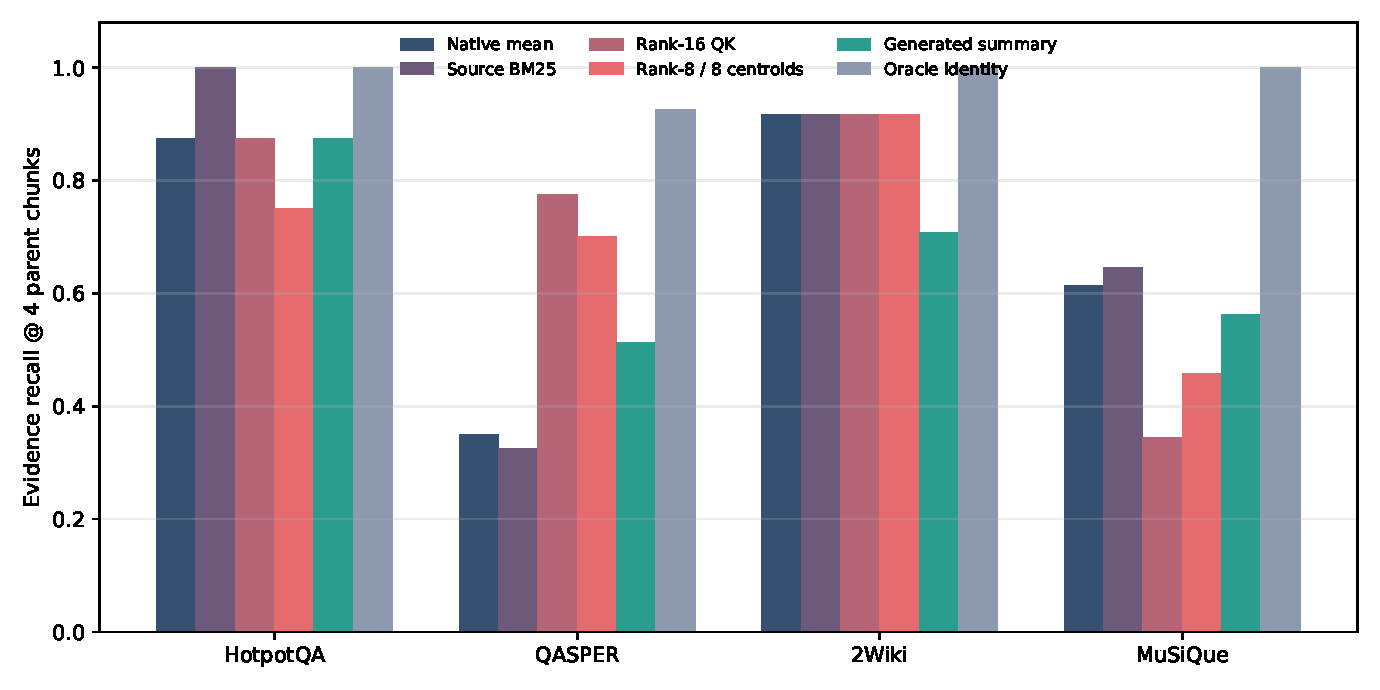
\includegraphics[width=\linewidth]{../shared/results/paper3_1_summary_index/publication/headline_recall.pdf}
\caption{Held-out evidence recall at four selected parent chunks. ``Generated summary'' denotes the scorer and generator frozen independently for each dataset on validation identities.}
\label{fig:headline}
\end{figure}

\begin{table}[H]
\centering
\small
\setlength{\tabcolsep}{3.4pt}
\begin{tabular}{lrrrrrrrr}
\toprule
Dataset & $n$ & Mean & Src. BM25 & R16 & R8/C8 & Summary & Oracle & $\Delta$ [95\% CI]\\
\midrule
HotpotQA & 4 & .875 & 1.000 & .875 & .750 & .875 & 1.000 & .000 [-.375,.375]\\
QASPER & 8 & .350 & .325 & .775 & .700 & .513 & .925 & +.163 [-.400,.688]\\
2Wiki & 4 & .917 & .917 & .917 & .917 & .708 & 1.000 & -.208 [-.417,.000]\\
MuSiQue & 8 & .615 & .646 & .344 & .458 & .563 & 1.000 & -.052 [-.375,.208]\\
\bottomrule
\end{tabular}
\caption{Evidence recall at matched selected-chunk budget. $\Delta$ is the paired summary-minus-native-mean effect. R16 and R8/C8 are inherited learned native-QK selectors.}
\label{tab:headline}
\end{table}

Complete recovery follows the same pattern. The summary policies recover every evidence chunk on $0.750$, $0.375$, $0.500$, and $0.250$ of HotpotQA, QASPER, 2Wiki, and MuSiQue examples. Thus the QASPER recall gain is not merely a partial-hit artifact, but it also does not close the oracle gap.

\section{Omission and addressability}

Natural retrieval cannot reveal whether a chunk was missed because the generator omitted an address or because the scorer failed to use one. We therefore construct 20 examples, four per fact type. Each example contains six topical chunks. One chunk hides a query-critical entity, alias, relation, date/number, or rare string as a minor detail. The target does not influence summary generation.

The full-source BM25 and the 32-token entity/rare-term extractive index recover every target chunk. The 0.6B retrieval summary also recovers all relation, date/number, and rare-string chunks, but only $0.75$ of entity chunks and $0.25$ of alias chunks. Crucially, it retains no complete target literal in any fact category. Retrieval sometimes succeeds because other generated wording correlates with the positive chunk; the shuffled-address control confirms that small-cohort ties and shared topical language can also produce nonzero recall.

\begin{figure}[t]
\centering
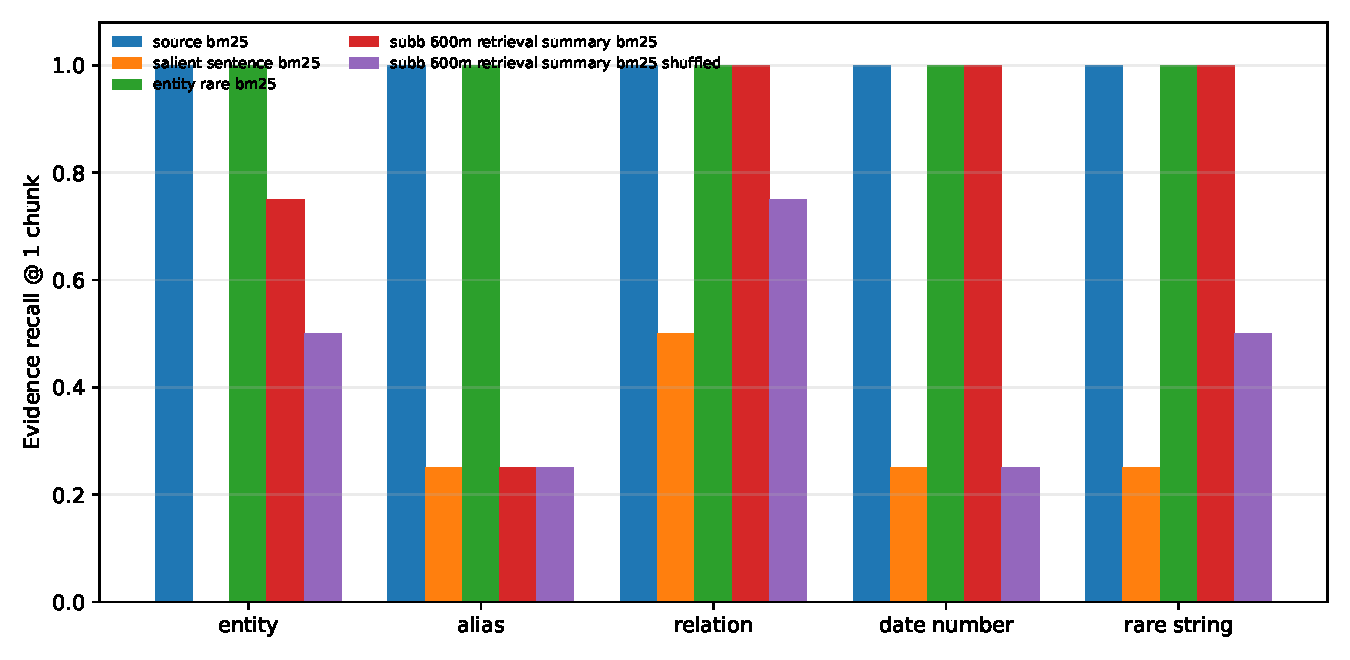
\includegraphics[width=.9\linewidth]{../shared/results/paper3_1_summary_index/publication/omission_recall.pdf}
\caption{Controlled low-salience fact retrieval at one selected chunk. A parameter-free entity/rare-term sidecar is both smaller and more reliable than generated summaries on this literal-address task.}
\label{fig:omission}
\end{figure}

The failure is conceptual rather than merely linguistic. A summary can be faithful while deleting the only future retrieval key. Retrieval-oriented prompting helps preserve classes of information, but a fixed 32-token language channel cannot guarantee coverage of every unknown discriminator. This supports a typed design: retain a lexical or entity sidecar for exact reachability and use summaries for paraphrastic or relational access.

\subsection{Natural address-preservation diagnostics}

We apply deterministic diagnostics to the held-out positive source parents.
Regex entities, numbers/dates, source-local rare terms, relation terms, and
query-overlapping evidence keys are measured against the frozen summary text.
Aliases are omitted because these natural cohorts do not provide independent
chunk-level alias labels. Figure~\ref{fig:address-retention} shows substantial
dataset heterogeneity and generally low literal preservation. Across available
positive parents, summaries retain only \PaperThreeOneEvidenceKeyRetention{} of
query-overlapping evidence keys.

\begin{figure}[t]
\centering
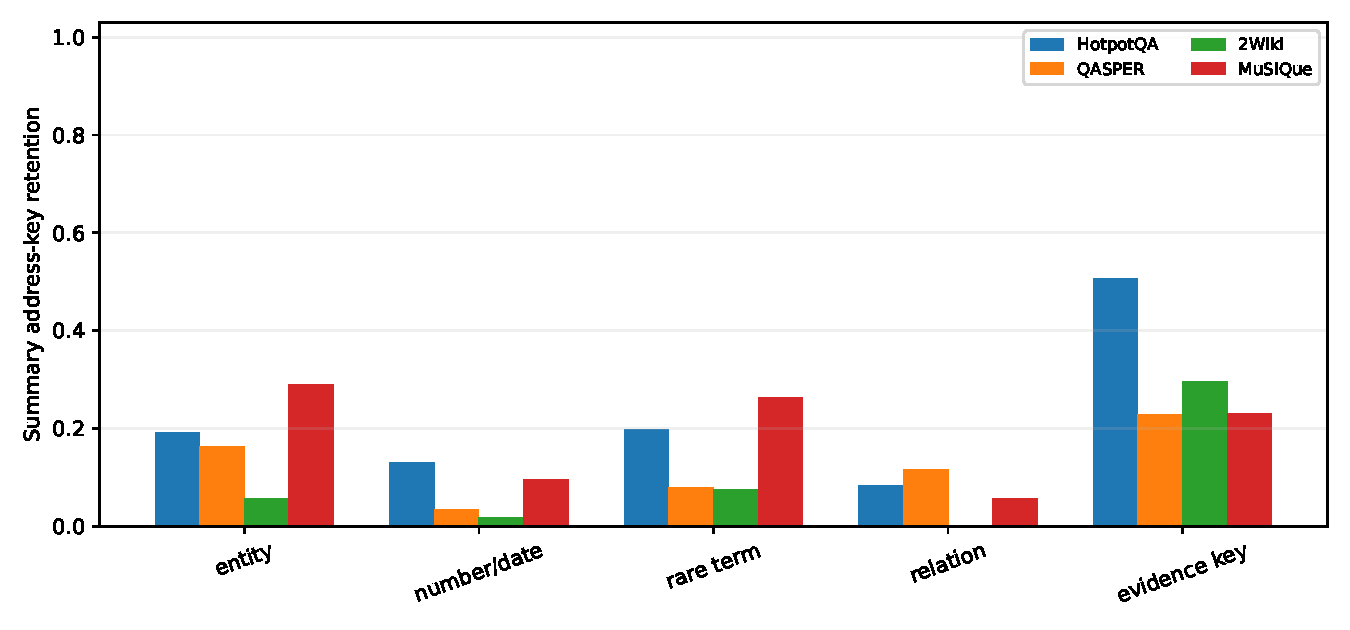
\includegraphics[width=.92\linewidth]{../shared/results/paper3_1_summary_index/multi_index/summary_address_retention.pdf}
\caption{Deterministic address-key retention in frozen summaries of positive
source parents. Missing reference categories are excluded rather than scored as
zero.}
\label{fig:address-retention}
\end{figure}

Evidence-key retention is the strongest measured descriptive predictor of
summary recovery, with pooled Spearman
$\rho=\PaperThreeOneEvidenceKeyCorrelation$ for target recovery at four. The
unit here is a positive source parent, so this is a diagnostic association, not
an independently powered inferential result. Figure~\ref{fig:quality-correlation}
also shows that length and compression ratio correlate with recovery, consistent
with a capacity--coverage tradeoff rather than a generic fluency deficit.

\begin{figure}[t]
\centering
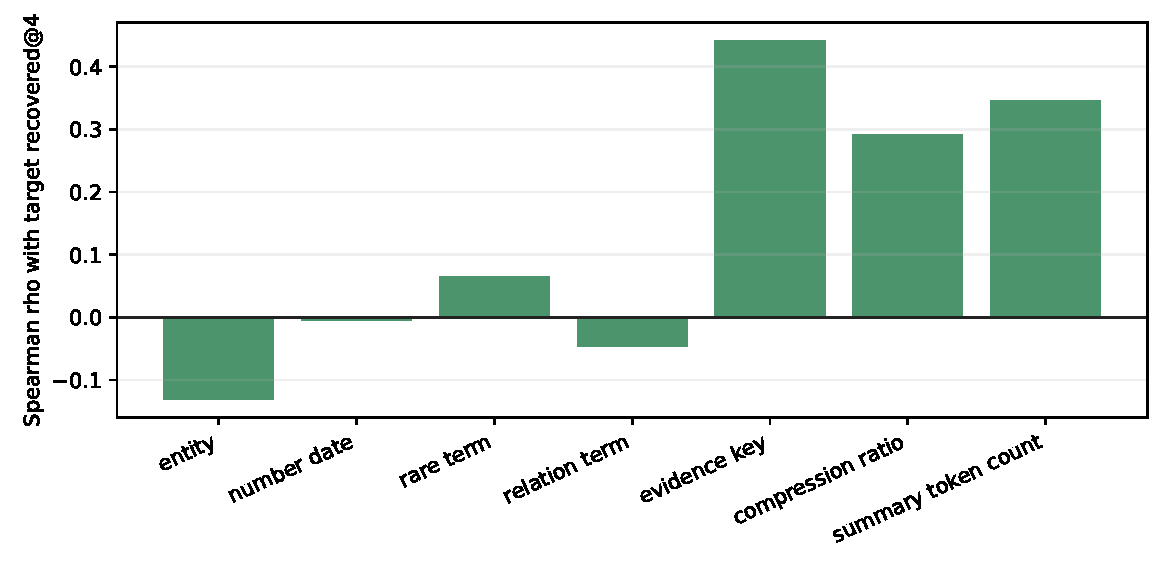
\includegraphics[width=.83\linewidth]{../shared/results/paper3_1_summary_index/multi_index/summary_quality_retrieval_correlation.pdf}
\caption{Pooled descriptive correlation between address diagnostics and
summary target recovery. Positive values mean higher diagnostic values tend to
coincide with recovery.}
\label{fig:quality-correlation}
\end{figure}

We do not report ROUGE, BLEU, or BERTScore. None of the four datasets supplies
an independently authored chunk-level retrieval-summary reference for these
records. Comparing a generated address against its full source and calling the
result conventional summary quality would mostly remeasure lexical coverage
and compression. The direct address-retention and retrieval correlations are
better aligned with the question tested here.

This distinction suggests three omission regimes. In \emph{explicit-answer
omission}, the query names a missing fact and can therefore trigger direct
recovery. In \emph{latent-evidence omission}, the missing fact is necessary but
is not itself named. In \emph{action-trigger omission}, the omitted fact would
have made a different tool or action relevant. The controlled benchmark
directly tests the second regime. It motivates the third, but does not measure
agent action selection.

\section{Fixed-budget multi-index competition}

\subsection{The channels are complementary}

Figure~\ref{fig:multi-overlap} classifies each evidence parent by which
single-channel top-four lists recover it. All eight HotpotQA evidence parents
are multi-channel recoveries. QASPER is less redundant: QK alone recovers four
evidence parents, $S$ alone recovers \PaperThreeOneSummaryUniqueQasper{}, $L$
alone recovers one, and six are missed by every channel. MuSiQue has
\PaperThreeOneSummaryUniqueMusique{} summary-only, two lexical-only, and one
extractive-only recovery. Summaries therefore contain unique routing signal;
the remaining question is whether that signal survives competition for four
slots.

\begin{figure}[t]
\centering
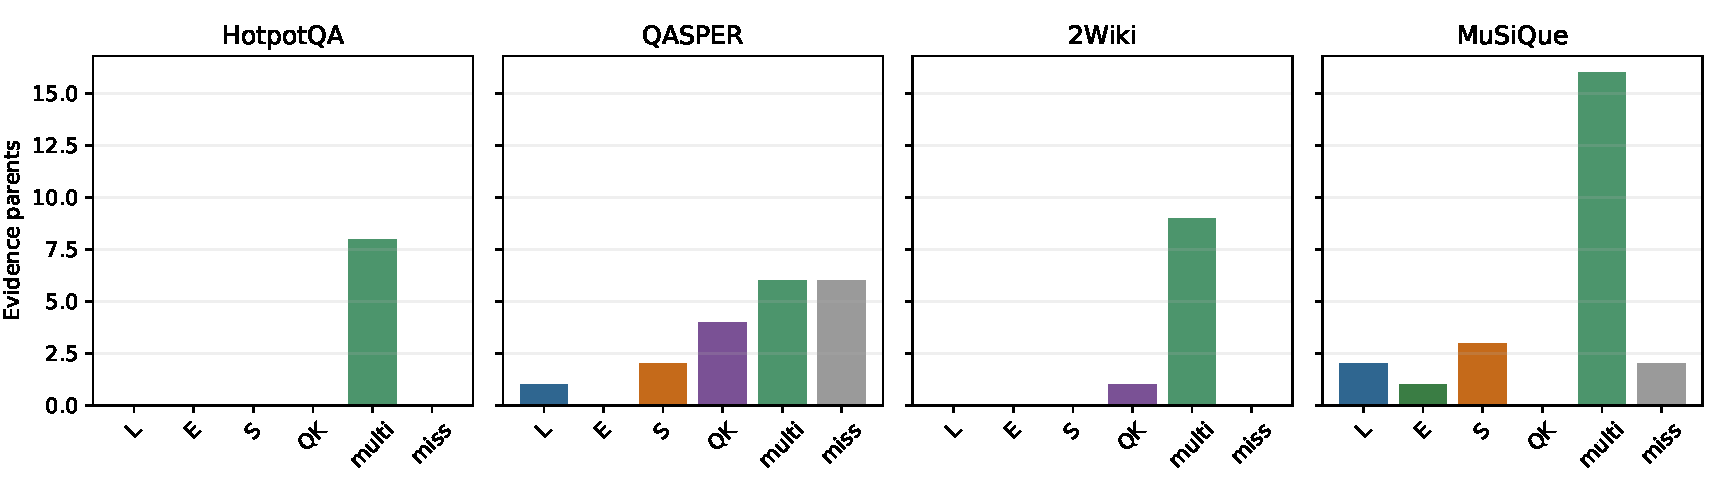
\includegraphics[width=\linewidth]{../shared/results/paper3_1_summary_index/multi_index/multi_index_channel_overlap.pdf}
\caption{Evidence-parent recovery by single-channel top-four lists. ``Multi''
means at least two of $L,E,S,QK$ recover the parent; ``miss'' means none does.
Counts describe complementarity before a combined admission policy.}
\label{fig:multi-overlap}
\end{figure}

\subsection{More address views do not imply more admitted evidence}

Table~\ref{tab:multi-main} reports the validation-frozen RRF comparison at the
same $K=4$ materialization budget. $L+S$ matches or exceeds either member on
HotpotQA and MuSiQue, and $L+QK$ reaches $1.000$ on 2Wiki. The full four-view
stack does not dominate. It ties the $L+E+QK$ base on HotpotQA and MuSiQue,
falls on QASPER, and loses one 2Wiki evidence outcome. The cost frontier in
Figure~\ref{fig:multi-frontier} makes the architectural accounting explicit:
these are multiple resident address views over one backing memory, not multiple
copies of native \kv.

\begin{table}[H]
\centering
\small
\resizebox{\linewidth}{!}{\begin{tabular}{lrrrr}
\toprule
Policy & HotpotQA & QASPER & 2Wiki & MuSiQue \\
\midrule
L & 1.000 & 0.325 & 0.917 & 0.646 \\
E & 0.875 & 0.138 & 0.917 & 0.552 \\
S & 0.875 & 0.512 & 0.708 & 0.562 \\
QK & 0.875 & 0.775 & 0.917 & 0.344 \\
L+S (RRF) & 1.000 & 0.475 & 0.917 & 0.688 \\
L+QK (RRF) & 1.000 & 0.588 & 1.000 & 0.542 \\
L+E+QK (RRF) & 1.000 & 0.588 & 1.000 & 0.573 \\
L+E+S+QK (RRF) & 1.000 & 0.475 & 0.917 & 0.573 \\
\bottomrule
\end{tabular}
}
\caption{Held-out evidence recall at $K=4$. Single-channel rows use their own
rankings. Combined rows use validation-frozen RRF and the same final parent
budget.}
\label{tab:multi-main}
\end{table}

\begin{figure}[t]
\centering
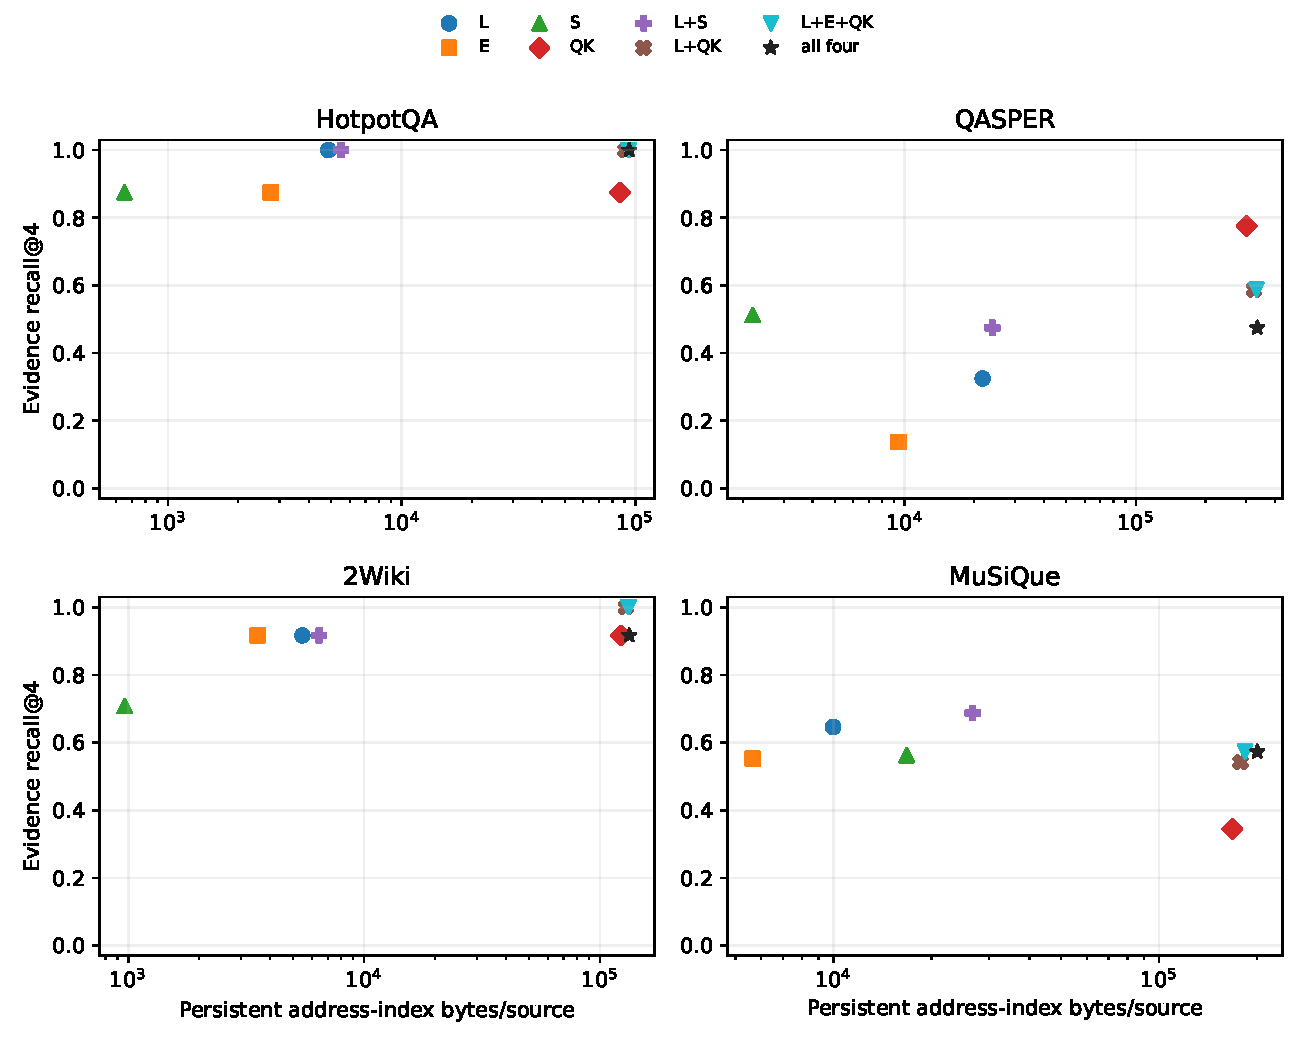
\includegraphics[width=.93\linewidth]{../shared/results/paper3_1_summary_index/multi_index/multi_index_recall_cost_frontier.pdf}
\caption{Fixed-budget recall versus persistent address-index bytes per source.
Backing source/native-\kv storage is shared and excluded from every point.}
\label{fig:multi-frontier}
\end{figure}

\subsection{Standalone value is not marginal value}

The primary marginal test is
\[
\Delta_S=R(L+E+S+QK)-R(L+E+QK).
\]
Here $R(\cdot)$ is evidence recall at the shared four-parent budget. The base
condition already has lexical ($L$), typed extractive ($E$), and learned QK
addresses. The difference therefore measures the summary's net contribution
after both unique recoveries and displaced base candidates are counted.

Under RRF, Table~\ref{tab:summary-marginal} gives deltas of
$\PaperThreeOneHotpotRrfSummaryDelta$,
$\PaperThreeOneQasperRrfSummaryDelta$,
$\PaperThreeOneTwoWikiRrfSummaryDelta$, and
$\PaperThreeOneMusiqueRrfSummaryDelta$. No positive interval excludes zero.
QASPER has one win, six ties, and one loss; the negative mean comes from the
larger loss. On 2Wiki, one loss and three ties produce the $-0.083$ delta.

\begin{table}[H]
\centering
\small
\begin{tabular}{lrrrr}
\toprule
Dataset & Base & +Summary & $\Delta_S$ & 95\% CI \\
\midrule
HotpotQA & 1.000 & 1.000 & +0.000 & [+0.000, +0.000] \\
QASPER & 0.588 & 0.475 & -0.113 & [-0.375, +0.037] \\
2Wiki & 1.000 & 0.917 & -0.083 & [-0.250, +0.000] \\
MuSiQue & 0.573 & 0.573 & +0.000 & [+0.000, +0.000] \\
\bottomrule
\end{tabular}

\caption{Summary marginal recall under validation-frozen RRF. ``Base'' is
$L+E+QK$; ``+Summary'' is $L+E+S+QK$. Intervals use 10,000 paired identity
resamples.}
\label{tab:summary-marginal}
\end{table}

Other admission rules reveal small but unresolved positive regimes. Round-robin
changes QASPER by $\PaperThreeOneQasperRoundRobinSummaryDelta$
$[\PaperThreeOneQasperRoundRobinLow,\PaperThreeOneQasperRoundRobinHigh]$ and
MuSiQue by $\PaperThreeOneMusiqueRoundRobinSummaryDelta$
$[\PaperThreeOneMusiqueRoundRobinLow,\PaperThreeOneMusiqueRoundRobinHigh]$.
A fixed $2L+2S$ MuSiQue reservation reaches
$\PaperThreeOneMusiqueReservedRecall$, a
$\PaperThreeOneMusiqueReservedDelta$ effect versus $L$ alone, but its interval
$[\PaperThreeOneMusiqueReservedLow,\PaperThreeOneMusiqueReservedHigh]$ also
crosses zero. Agreement priority and normalized fusion likewise fail to produce
a resolved positive summary marginal. Full policy grids appear in
Appendix~\ref{app:admission}.

The distinction matters. Summaries are \emph{complementary}: they find evidence
missed by $L,E,$ and $QK$. They do not yet show \emph{net fixed-budget utility}
because unconditional admission can displace stronger candidates. Selective
summary admission remains plausible; a default four-view union does not.

\begin{figure}[H]
\centering
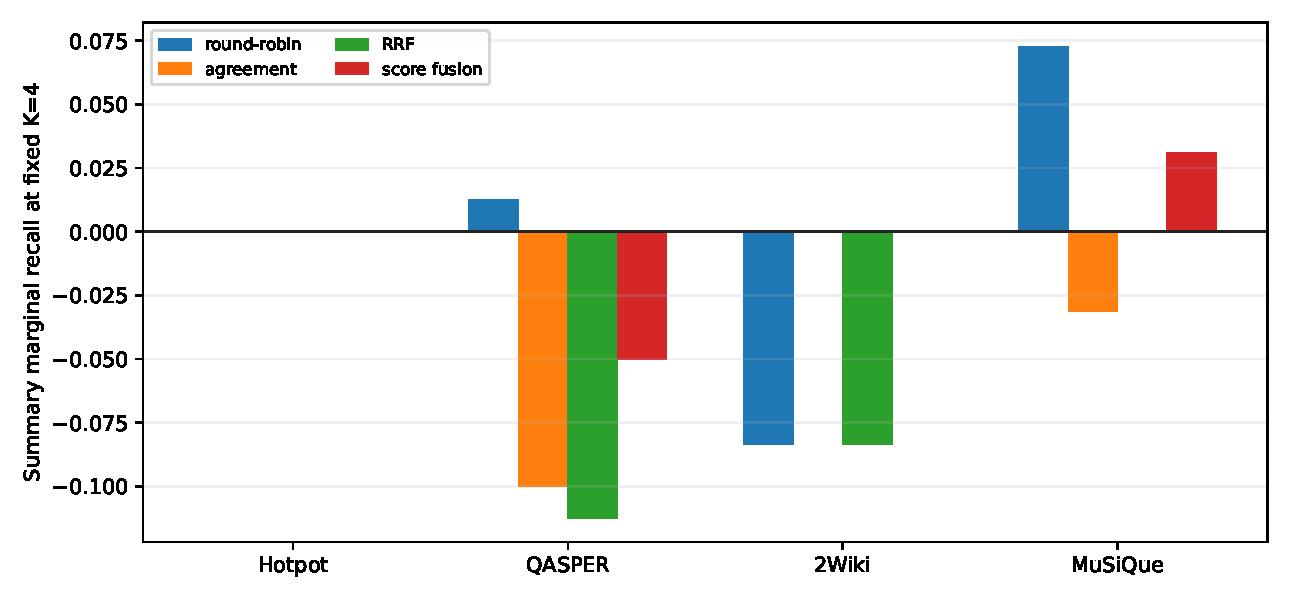
\includegraphics[width=.9\linewidth]{../shared/results/paper3_1_summary_index/multi_index/summary_marginal_contribution.pdf}
\caption{Summary marginal recall across four fixed admission families. All
comparisons hold $K=4$ constant.}
\label{fig:summary-marginal}
\end{figure}

\section{Cost}

\subsection{Storage and time accounting}

Table~\ref{tab:cost} separates the persistent routing index from backing source/native-\kv storage and from the physically materialized native \kv. Pure lexical summary policies occupy only $652$--$2{,}205$ bytes per source. MuSiQue's selected hybrid occupies $16{,}793$ bytes because $15{,}744$ bytes are frozen embedding vectors; summary text itself occupies about $1{,}049$ bytes. None of these numbers includes backing native memory.

\begin{table}[H]
\centering
\small
\begin{tabular}{lrrrrrr}
\toprule
Dataset & Index B & Emb. B & Tokens & Ingest s & Route ms & Native tokens\\
\midrule
HotpotQA & 652 & 0 & 166 & 131.1 & 0.186 & 1020\\
QASPER & 2205 & 0 & 483 & 46.6 & 0.561 & 1020\\
2Wiki & 966 & 0 & 240 & 176.8 & 0.453 & 904\\
MuSiQue & 16793 & 15744 & 280 & 25.3 & 371.4 & 903\\
\bottomrule
\end{tabular}
\caption{Mean per-source accounting for each frozen summary policy. ``Index B'' includes embedding bytes when the selected scorer requires them. Native tokens are materialized after routing and remain governed by the common four-parent budget.}
\label{tab:cost}
\end{table}

Table~\ref{tab:multi-cost} reports the combined resident indices. The base
stack stores lexical text, the typed extractive sidecar, and rank-16 QK once.
Adding $S$ charges only summary text and, for MuSiQue, its frozen embedding.
The shared backing source/native-\kv record is counted once in both conditions.
Summary generation dominates one-time ingestion even when its persistent byte
increment is small. QK projection/index construction is inherited from the
frozen Paper 2.8 artifacts and is marked as not remeasured rather than assigned
a zero-cost claim.

\begin{table}[H]
\centering
\small
\begin{tabular}{lrrr}
\toprule
Dataset & Base bytes & +Summary bytes & Summary ingestion (s) \\
\midrule
HotpotQA & 93621 & 94273 & 131.1 \\
QASPER & 332221 & 334426 & 46.6 \\
2Wiki & 131886 & 132852 & 176.8 \\
MuSiQue & 183568 & 200361 & 25.7 \\
\bottomrule
\end{tabular}

\caption{Mean persistent address bytes and measured summary ingestion time per
source. ``Base'' is $L+E+QK$ and ``+Summary'' is $L+E+S+QK$. Both use one shared
native-memory backing record.}
\label{tab:multi-cost}
\end{table}

For $Q$ later queries to one source, measured one-time generation $C_s$ contributes $C_s/Q$ seconds per query. At $Q=1000$, that term is $0.131$, $0.047$, $0.177$, and $0.025$ seconds for HotpotQA, QASPER, 2Wiki, and MuSiQue. Considering routing time alone, generation amortizes against native-mean scoring after approximately $479{,}000$, $25{,}800$, and $7{,}300$ queries on the first three datasets. MuSiQue's external embedding route is slower and never breaks even in this local implementation. Against source BM25, the corresponding thresholds are about $70{,}000$, $9{,}800$, $171{,}000$, and never.

These are not favorable end-to-end break-even claims. The conditions with lower routing cost do not also provide a reliable quality gain. The measurements instead establish the scale at which asynchronous ingestion could become acceptable for repeatedly queried, stable corpora.

\subsection{Gate decisions and implications}

\paragraph{Frozen concept gate.}
QASPER shows standalone summary value, and channel-overlap rows confirm unique
summary recoveries on QASPER and MuSiQue. The stricter marginal gate remains
closed: adding $S$ to $L+E+QK$ produces no resolved positive effect under RRF,
round-robin, agreement, or normalized fusion. We therefore classify summaries
as optional candidate sources rather than members of the default resident
stack.

\paragraph{Teacher and training gate.}
The 8B teacher does not establish general headroom: it ties on held-out HotpotQA and regresses on 2Wiki. More importantly, the frozen summary has no reliable marginal value after stronger companion views are present. Training a LoRA summarizer would consequently optimize into a weak and dataset-specific target. No LoRA distillation is run in this iteration.

\paragraph{Native-use gate.}
The identity projection, requested token counts, and unchanged materialization policy are verified, but no answer-likelihood or generation claim is made. The multi-index discovery gate is not strong enough to justify a downstream native-\kv study. Summary-only answering is also omitted because it would test a different text-RAG system after the relevant gate closed.

\paragraph{Architectural implication.}
The supported design is one immutable native-memory record with multiple typed
address views. Exact tokens, aliases, and identifiers remain with lexical or
extractive indices. Learned native-QK channels cover host-model geometry.
Generated summaries contribute inspectable relational language only when a
selective policy can justify a slot. The router deduplicates identities before
one common native-\kv materializer. The multi-index result replaces a vague
``hybrid'' recommendation with an explicit admission requirement: channel
complementarity is useful only when final-slot competition is calibrated.

\section{Related work}

The systems nearest to this study differ less in whether they retain the
original than in how omitted content becomes reachable again. That distinction
matters because \emph{nothing is permanently lost} does not imply that
\emph{everything remains discoverable at the decision point}.

\paragraph{Reversible context compression.}
Headroom applies type-aware compressors to tool outputs, database results, file
reads, logs, and retrieved text. Its Compress--Cache--Retrieve (CCR) path keeps
the original in a local cache, places a marker or handle in the compressed
view, and injects a \code{headroom\_retrieve} tool. On supported proxy paths,
the response handler resolves that tool transparently; the context tracker can
also re-expand relevant cached content proactively
\cite{headroomCCR,headroomArchitecture}. Type-specific handling preserves
structure and anomalies rather than forcing every record through one language
summary. The project's public reproducible benchmarks report large compression
on several structured outputs and favorable QA and extraction accuracy
\cite{headroomBenchmarks}. These are meaningful system results.

Paper 3.1 asks a different question. CCR makes the original recoverable once a
marker, model action, or tracker chooses the right cached object. We ask whether
a compact representation preserves the unknown-future address needed to make
that choice. The controlled benchmark supports concern about latent-evidence
omission; it does not show that Headroom fails, that CCR cannot recover an
original, or that its safety mechanisms are ineffective. Whether an omitted
detail changes a later tool decision is a hypothesis for a separate agent-level
study.

\paragraph{Prompt and selective compression.}
Selective Context prunes low-information units, while LLMLingua and
LongLLMLingua allocate compression budgets and remove tokens to reduce prompt
cost while preserving downstream performance
\cite{li2023selective,jiang2023llmlingua,jiang2023longllmlingua}. These methods
optimize the representation the model consumes. In contrast, a PRA summary is
not consumed as evidence. It is one address view whose selected identity
resolves to the original native representation. Conventional summary quality
can therefore diverge from address quality, especially for low-salience future
discriminators.

\paragraph{Agent memory and programmatic state.}
MemGPT moves information among model-managed memory tiers and uses explicit
control flow for retrieval \cite{packer2024memgpt}. Scroll instead keeps an
append-only event log and a typed persistent program environment; only printed
projections enter the working view, while eviction landmarks retain exact log
addresses \cite{lin2026scroll}. These systems preserve richer state and expose
recovery through model actions or programs. PRA is narrower: index scoring can
select an immutable source identity before the model emits a recovery action.
Scroll's landmarks are particularly close in spirit to identity-backed address
views, although its unit of consumption is a programmatically projected event
rather than selected native \kv.

\paragraph{Retrieval and KV selection.}
RAG retrieves external documents and places text in the generator's context
\cite{lewis2020rag}; lexical, dense, and hybrid variants mainly differ in how
documents are ranked. RetrievalAttention indexes key vectors and retrieves a
sparse subset of the KV cache during decoding \cite{liu2025retrievalattention}.
PRA combines these boundaries: lexical, extractive, generated, and learned-QK
views can all address the same source record, while a separate materializer
controls native-\kv consumption. The contribution here is not a new universal
retriever. It is the fixed-budget test showing that an additional address view
must earn scarce materialization slots.

\begin{table}[t]
\centering
\small
\begin{tabularx}{\linewidth}{p{.17\linewidth}p{.21\linewidth}p{.23\linewidth}X}
\toprule
System family & Losslessly retained & Initial model view & Recovery path \\
\midrule
Headroom CCR & Cached original & Type-compressed output and marker & Model tool, proxy handler, or proactive tracker \\
MemGPT / Scroll & Memory tier or event log & Active tier or printed projection & Model-managed memory action or program \\
Text RAG & External document corpus & Retrieved passages & Lexical, dense, or hybrid retriever \\
Prompt compression & Usually source outside compressed prompt & Pruned or rewritten text & Usually no identity-bound recovery path \\
PRA here & Source identity and native \kv backing & Compact typed addresses & Indexed selection, then identity-resolved native \kv \\
\bottomrule
\end{tabularx}
\caption{The decisive comparison is not only what remains stored, but what
causes omitted content to become visible when a later decision needs it.}
\label{tab:related-taxonomy}
\end{table}

\section{Limitations}

The held-out natural cohorts contain only 24 identities, and two teacher
datasets contain four identities each. Bootstrap intervals appropriately remain
wide. Multi-index fusion choices use only two validation identities per
dataset; the tiny grid limits overfitting but cannot make policy selection
stable. The primary conclusion is specific to a fixed four-parent budget.
Larger or adaptive budgets could change which channels are marginally useful.
The equal-budget geometry study is a two-identity validation diagnostic. The
omission benchmark is controlled and intentionally adversarial; its absolute
rates should not be generalized to natural corpora.

Generation uses local quantized Ollama models and one machine with a 4GB GPU. The 8B teacher is CPU/GPU split, so its latency should not be treated as a hardware-independent model benchmark. Peak ingestion memory was not sampled robustly; this paper reports wall time, persistent bytes, and model metadata instead. MiniLM timing includes local service overhead and is not an optimized in-process embedding implementation.

The study measures discovery, not final answer quality. Although selected
records map to unchanged native-memory requests, no downstream generation is
run after the gate closes. All evaluated summary addresses are model-generated;
there is no independently authored natural reference-summary set. Natural alias
labels are also unavailable. These omissions are why we report address-key
retention rather than ROUGE-style metrics. No learned controller decides when a
summary deserves a slot, so the negative unconditional result does not rule out
selective summary admission. The frozen cache caps output at 32 tokens;
extending it to 64 or 128 would require a new generation intervention, not a
post-hoc truncation comparison. Finally, the study does not compare directly
against Headroom, CCR, Scroll, or an agent action benchmark. Claims about
action-trigger omission remain hypotheses rather than measured failures of
those systems.

\section{Conclusion}

Natural-language summaries can be compact, inspectable routing addresses for native memory. They are not reliable universal addresses. In this pilot, one QASPER policy improves over a native mean key, and summaries uniquely recover several QASPER and MuSiQue evidence parents. Yet those unique candidates do not yield reliable marginal recall after lexical, typed extractive, and learned-QK views compete for the same four slots. Controlled omission and natural address diagnostics show the deeper reason: fluent compression can remove exactly the low-salience string that a future query needs.

The useful outcome is architectural clarity: one immutable native-memory record
can support several compact address views. Lexical and extractive views preserve
explicit reachability; QK preserves host-model geometry; summaries provide a
lossy, human-readable semantic address. Their scores must be combined by a
fixed-budget admission policy before selected identities resolve to unchanged
native \kv. The default stack remains $L+E+QK$. Summary routing is an optional
experimental channel until larger cohorts demonstrate positive marginal value;
only then should learned summarization or downstream generation reopen.

The experiments and claims are now frozen for external review. Reopening the
mechanism requires either a validity correction or an independently powered
test of selective marginal utility.

\appendix

\section{Generator and scorer frontier}
\label{app:frontier}

The generated-model frontier contains 135M, 0.6B, 1.2B, 4B, and 8B local
models. Generation prompts are either generic summaries or retrieval-oriented
addresses, with one or several facets under a fixed maximum token budget. The
same generated text is scored independently by normalized token overlap, BM25,
frozen MiniLM cosine similarity, or a convex fusion. For the hybrid scorer,
each channel is min--max normalized within one source before
\[
r_i^{\mathrm{hyb}}
=\alpha\widetilde r_i^{\mathrm{BM25}}
 +(1-\alpha)\widetilde r_i^{\mathrm{emb}}.
\]
Validation considers only $\alpha\in\{0.25,0.50,0.75\}$. Faceted records score
each facet separately and assign the parent its maximum facet score. Generator,
prompt, facet geometry, scorer, and fusion weight are frozen before held-out
evaluation.

\section{Cache safety and provenance}
\label{app:cache}

The generation cache key hashes the model, prompt version, token budget, facet
count, and exact source text. It excludes the logical item identifier so that
identical source text can reuse generated content. Reuse never reuses identity:
a cache hit is rebound to the requesting URI, parent identifier, token span,
and source hash. Before evaluation, \code{assert\_source\_alignment()} compares
the complete identity set with the inherited native-memory registry. A
duplicate-content regression test verifies that cache reuse cannot alias two
native-memory records.

\section{Equal-budget facet geometry}
\label{app:facets}

Facets might spread a fixed generation budget across independent addresses. We
compare $1\times32$, $2\times16$, $4\times8$, and $8\times4$ maximum-token
geometries with a frozen 1.2B model on two HotpotQA validation identities. BM25
recall is $0.50$, $0.75$, $0.50$, and $0.50$, respectively. The small
diagnostic favors two medium facets, not monotonically more facets.

\begin{figure}[H]
\centering
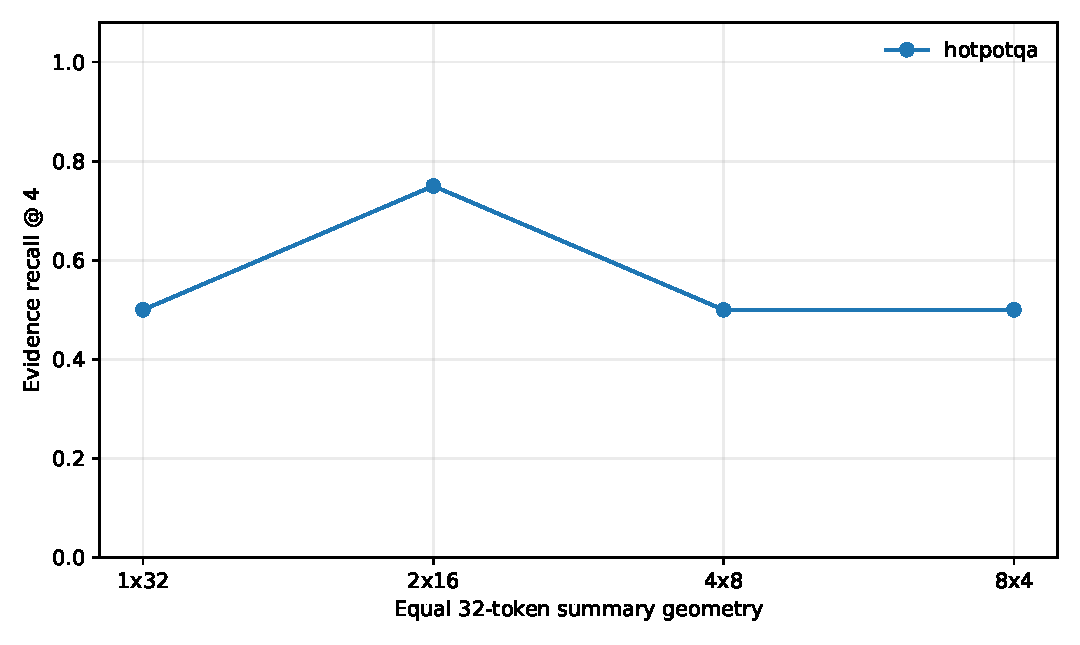
\includegraphics[width=.72\linewidth]{../shared/results/paper3_1_summary_index/publication/geometry_recall.pdf}
\caption{Diagnostic equal-budget facet geometry on two validation identities;
it is not a held-out cross-dataset result.}
\label{fig:geometry}
\end{figure}

Actual output is shorter than the maximum: the four geometries use 184, 172,
151, and 152 summary tokens per source across all candidate chunks. Ingestion
takes 33.7, 33.4, 47.9, and 48.9 seconds per source. Structured-output overhead
therefore makes many short facets more expensive even at equal content-token
capacity.

\section{Multi-index admission grid}
\label{app:admission}

The matrix includes every channel pair, selected three-channel stacks, and
$L+E+S+QK$. Round-robin and agreement union are parameter-free. Reserved
policies include $2L+2S$, $2E+2S$, $2L+2QK$, $2E+2QK$, and one- or two-slot
lexical safety reservations. Normalized fusion searches only equal,
address-weighted, semantic-weighted, summary-weighted, and QK-weighted
templates. RRF searches $d\in\{10,60\}$. Each choice is frozen separately by
dataset and channel set on validation identities. Candidate scores, ranks,
admitted identities, and wins/ties/losses are retained in the row-level
artifacts.

\section{Extended diagnostics and tables}
\label{app:extended}

The tracked publication directory contains per-example recall, precision,
complete recovery, reciprocal rank, channel overlap, and paired effects for
every frozen standalone policy. The multi-index directory adds every union and
fusion row, policy-specific paired effects, channel-hit decomposition, and
address-retention diagnostics. Generated TeX tables are rebuilt from those
rows; numerical claims in the main text are not maintained by hand.

\section{Extended cost accounting}
\label{app:costs}

Cost artifacts separate persistent address bytes, embedding bytes, generated
tokens, one-time ingestion wall time, routing wall time, backing source/native
memory, and physically materialized native tokens. The base and summary-added
conditions share one backing record. QK projection cost is inherited and
marked unmeasured in this replay; it is never assigned a zero. Amortization
tables report $C_s/Q$ for repeated queries rather than treating ingestion as a
per-query charge.

\section{Controlled omission construction}
\label{app:omission}

The omission benchmark contains 20 examples, four each for entities, aliases,
relations, dates or numbers, and rare strings. Six topically similar chunks
appear in each example. One low-salience fact identifies the positive chunk,
but the query is withheld during summary generation. Full-source BM25, the
typed extractive index, the generated-summary index, and a shuffled-address
control are evaluated at one admitted chunk. The construction tests latent
evidence omission, not natural prevalence and not downstream tool selection.

\section{Reproducibility}
\label{app:reproducibility}

Every row is tracked with dataset identity, selected and positive parent
indices, index bytes, generated tokens, ingestion and routing time, and
materialized native-\kv tokens. Manifests record source-model revision, Ollama
metadata, prompt version, generation and dataset seeds, inherited feature
hashes, and source commits. Generated addresses are append-only JSONL records;
source text and large native-QK tensors are not duplicated into the repository.

The original runner is
\code{experiments/paper3\_1\_summary\_index/run\_study.py}. The multi-index
replay is \code{run\_multi\_index\_study.py};
\code{build\_multi\_index\_artifacts.py} regenerates effects, tables, macros,
and figures. Focused tests cover source alignment, typed extraction,
deterministic unions, reservations, RRF, normalized fusion, native-request
projection, cache resumption, and duplicate-content rebinding.

\begin{thebibliography}{99}

\bibitem{headroomCCR}
Headroom Labs. Reversible Compression (CCR), 2026.
\url{https://docs.headroomlabs.ai/docs/ccr}.

\bibitem{headroomArchitecture}
Headroom Labs. Architecture: context routing, type-specific compression, and
CCR, 2026. \url{https://docs.headroomlabs.ai/docs/architecture}.

\bibitem{headroomBenchmarks}
Headroom Labs. Compression and accuracy benchmarks, 2026.
\url{https://docs.headroomlabs.ai/docs/benchmarks}.

\bibitem{li2023selective}
Yucheng Li, Bo Dong, Chenghua Lin, and Frank Guerin. Compressing context to
enhance inference efficiency of large language models. EMNLP, 2023.
\url{https://arxiv.org/abs/2310.06201}.

\bibitem{jiang2023llmlingua}
Huiqiang Jiang, Qianhui Wu, Chin-Yew Lin, Yuqing Yang, and Lili Qiu.
LLMLingua: Compressing prompts for accelerated inference of large language
models. EMNLP, 2023. \url{https://arxiv.org/abs/2310.05736}.

\bibitem{jiang2023longllmlingua}
Huiqiang Jiang, Qianhui Wu, Xufang Luo, Dongsheng Li, Chin-Yew Lin, Yuqing
Yang, and Lili Qiu. LongLLMLingua: Accelerating and enhancing LLMs in long
context scenarios via prompt compression. ICLR, 2024.
\url{https://arxiv.org/abs/2310.06839}.

\bibitem{packer2024memgpt}
Charles Packer, Sarah Wooders, Kevin Lin, Vivian Fang, Shishir G. Patil, Ion
Stoica, and Joseph E. Gonzalez. MemGPT: Towards LLMs as operating systems,
2024. \url{https://arxiv.org/abs/2310.08560}.

\bibitem{lin2026scroll}
Yin Lin, Elaine Ang, Erkang Zhu, Bolin Ding, and Jingren Zhou. Context as an
environment: Programmatic context management for long-horizon agents, 2026.
\url{https://arxiv.org/abs/2608.21690}.

\bibitem{lewis2020rag}
Patrick Lewis et al. Retrieval-augmented generation for knowledge-intensive
NLP tasks. NeurIPS, 2020. \url{https://arxiv.org/abs/2005.11401}.

\bibitem{liu2025retrievalattention}
Di Liu et al. RetrievalAttention: Accelerating long-context LLM inference via
vector retrieval. NeurIPS, 2025.
\url{https://arxiv.org/abs/2409.10516}.

\end{thebibliography}

\end{document}
